\section{Electrochemical energy conversion and storage devices}

At last, we aim in the description of the main technologies allowing us to use the information about the electrochemical cells obtained so far in order to generate energy. In particular, we are going to focus on the description of: Galvanic devices, with the aim of generating potentials or currents such as batteries or fuel cells, Electrolytic, which uses electricity to perform particular reactions such as electrolysis cells or photochemical ones, and supercapacitors.

\subsection{Galvanic devices}

This type of devices are thought in order to generate electrical energy from chemical one, and both batteries and fuel cells achieve this result in two different ways. Nevertheless, such technologies are really powerful since are able to generate electricity directly from chemical reactions, basically skipping the steps of generating heat, transforming it in mechanical energy and then create electrical one that classical transformer used. This leads batteries and fuel cells to have theoretical efficiencies that are much higher and not limited by the Carnot one. Still, the two methods differ on a general level since the batteries are based on pure electrochemical cells, meaning that are \textbf{closed systems}, while the fuel cells uses Hydrogen as electrode that needs to be inserted as gas, leading to the need for an \textbf{open system}.

Before diving into the particular description of batteries architecture we can tell some general considerations about Galvanic devices. In particular, it's important to keep in mind that inside a general Galvanic cell the system can be \textbf{charged} or \textbf{discharged} so that the electric energy can be stored or taken by the system, respectively. Nevertheless, the discharge of the system is spontaneous, since the cell is thought as so, while the charge needs an external bias in order to happen so that $E > E_{eq}$, where $E_{eq}$ is the potential of the cell. Therefore, by using a bias we are able to switch the role of the electrodes, going from discharge to charge, but the \textbf{polarity doesn't change} that should not be touched. Another general important thing to take into account is the fact that as the reaction goes on the concentration of the oxidated and reduced species inside the electrolyte changes, changing also the activities of the species which modifies $E_{eq}$. To make an example we can see the case of a Cu-Zn cell where by using Nernst equation we can use
\begin{equation}
    E_{eq} = E^0_{cell} + \frac{RT}{nF}\ln\left( \frac{a_{Cu^{2+}}}{a_{Cu}} \right) - \frac{RT}{nF}\ln\left( \frac{a_{Zn^{2+}}}{a_{Zn}} \right).
\end{equation}
Nevertheless, we can also use the fact that Cu and Zn are metals so that their activities are taken as $\sim 1$ so that we can write
\begin{equation}
    E_{eq} = E^0_{cell} + \frac{RT}{nF}\ln\left( \frac{a_{Cu^{2+}}}{a_{Zn^{2+}}} \right),
\end{equation}
where the activities are functions of the molar fractions, as we know, so that as the reaction goes on the cell potential changes, generally \textbf{decreasing while discharging} and \textbf{increasing while charging}. Still, the variation that the activity change bring to the potential is not large, due to the logarithmic dependence, allowing for the potential to be considered nearly constant in applications. Keeping those things in mind we can try to focus on the description of the main devices in this category.

\paragraph{Batteries.} A battery is defined simply as a system composed by 2 or more cells connected together so that the cell potential is defined by the sum of the ones of the different cells. Such devices are also divided in two main types: \textbf{primary}, that can't be recharged, and \textbf{secondary}, with the possibility of use it more times by recharging. I'm not going to write here all the different types of possible batteries, just keep in mind that the one based on Litium is better than the other thanks to the really high ionization potential of Li and its low mass that allows for a large limiting current inside the cell. What is interesting are the possible process used to design a cell, for example a possibility is the \textbf{reconstruction reaction} process, where the cells use simple electrodes that get deteriorated or reconstructed upon charge or discharge. In this case we have that the cell is a primary one if the results of the reaction is soluble inside the solution, since in the case where the result deposit inside the solution through an irreversible reaction it's not possible to go back, so obviously no recharge can be done. Still, there are also cases where the recharge is not possible even for reversible situations, for example Litium has a problem with this type of batteries since during the charge process it gets deposited on the electrode in an inhomogeneous way creating structure that grows inside the cell called dendrites. Such structure can eventually grow to the point that touches also the other electrode creating a circuit that heats the solution increasing the volume destroying the cell. That is a great safety problem since Litium is highly reactive with air and when the circuit breaks the Litium touches it and takes fire, which is a big problem especially on planes. Nevertheless, the problem can be overcomed by the use of the \textbf{insertion reaction} design, where the ions do not come from electrodes made of metallic plates of the wanted element but inside specific containers, such as graphite layers, that can also have a role in the reaction changing valence number. Still, such design eliminates the need of metal plates highly increasing the safety of the technology since problems such as dendrites cannot happen, but other ones are still present such as volume changes or phase transitions that can happens due to change in concentration inside the solution that can break the batteries and generate the same battery destruction problem as before, but with less probability.
\begin{figure}[t]
    \centering
    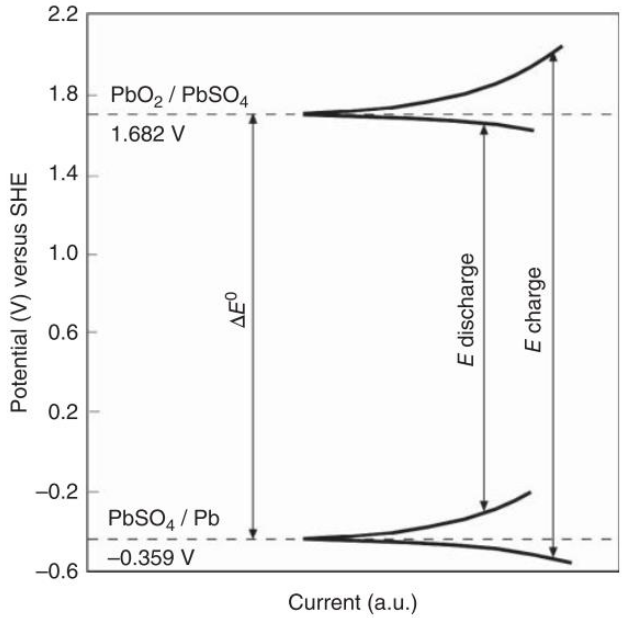
\includegraphics[width=0.33\textwidth]{Immagini/CellPotVar.png}
    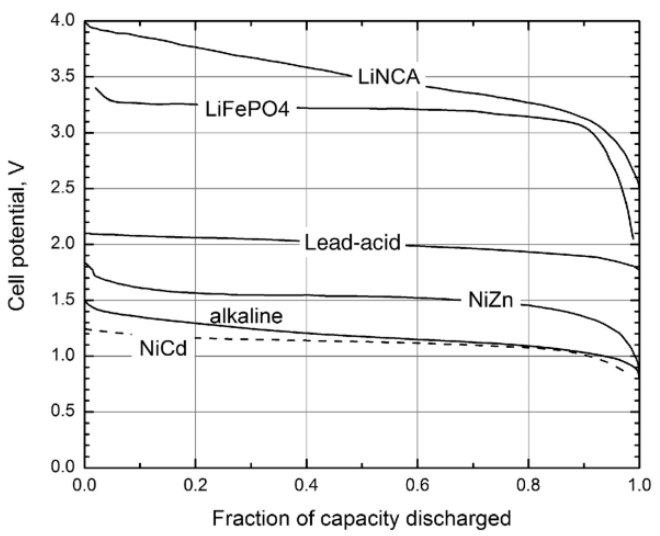
\includegraphics[width=0.4\textwidth]{Immagini/CellSpec.png}
    \caption{
        Graphical representation of the variation of the potential for a Galvanic cell as the reactions goes on, showing how effectively changes increasing for charge and decreasing for discharge, to the left. To the right, instead, some specific of certain batteries.
    }
    \label{fig:CellSpec}
\end{figure}

In order to tell when a battery is better that the others we need to create some specific quantities that we can look at. Such quantities are usually taken as: the specific energy inside the battery, the volumetric energy, the C-rate and the cell polarization. The first two are only needed to understand how much energy is present inside a particular battery, and it's important since higher they are and smaller or lighter the devices can be. The other ones are more mathematics, for example the C-rate is defined as the current that the battery can sustain for one hour and then be totally without energy
\begin{equation}
    C = \frac{Q_{tot}}{1\text{h}}.
\end{equation}
So, if we have a $C = \SI{2.3}{A/h}$ then this means that we can sustain a current of \SI{0.23}{A} for \SI{10}{\hour} which is great to know. Still, the rate at which we draw power from the cell influences the cell potential since $E_{cell}$ is going to decay respect the $E_{eq}$ during the discharge to the point where is dropping to zero due to polarization
\begin{equation}
    E_{eq} - E_{cell} = \eta_{pol} = \abs{\eta_{ohm}} + \abs{\eta_{kin}} + \abs{\eta_{conc}}.
\end{equation}
Various contribution to this phenomenon are present, such as: \textbf{resistance polarization} due to the presence of a voltage drop thanks to solution resistance, \textbf{activation polarization} accounting for the kinetics of the charge transfer reaction described by Butler-Volmer relation, and \textbf{concentration polarization} arising from mass transport limitations that can be presents also for concentration gradients. All of them are important since the polarization itself needs to be taken into account inside the system due to the fact that generates heat. In fact, can be seen how heat generation in batteries can be written as
\begin{equation}
    \dot{q} = J\eta_{pol} - J\pdv{E}{T}[W],
\end{equation}
so that the first term is the leading one and is always positive generating heat, therefore the control over the polarization is really important.